\section{方法}
\label{sec:method}

\begin{figure*}[!t]
\centering
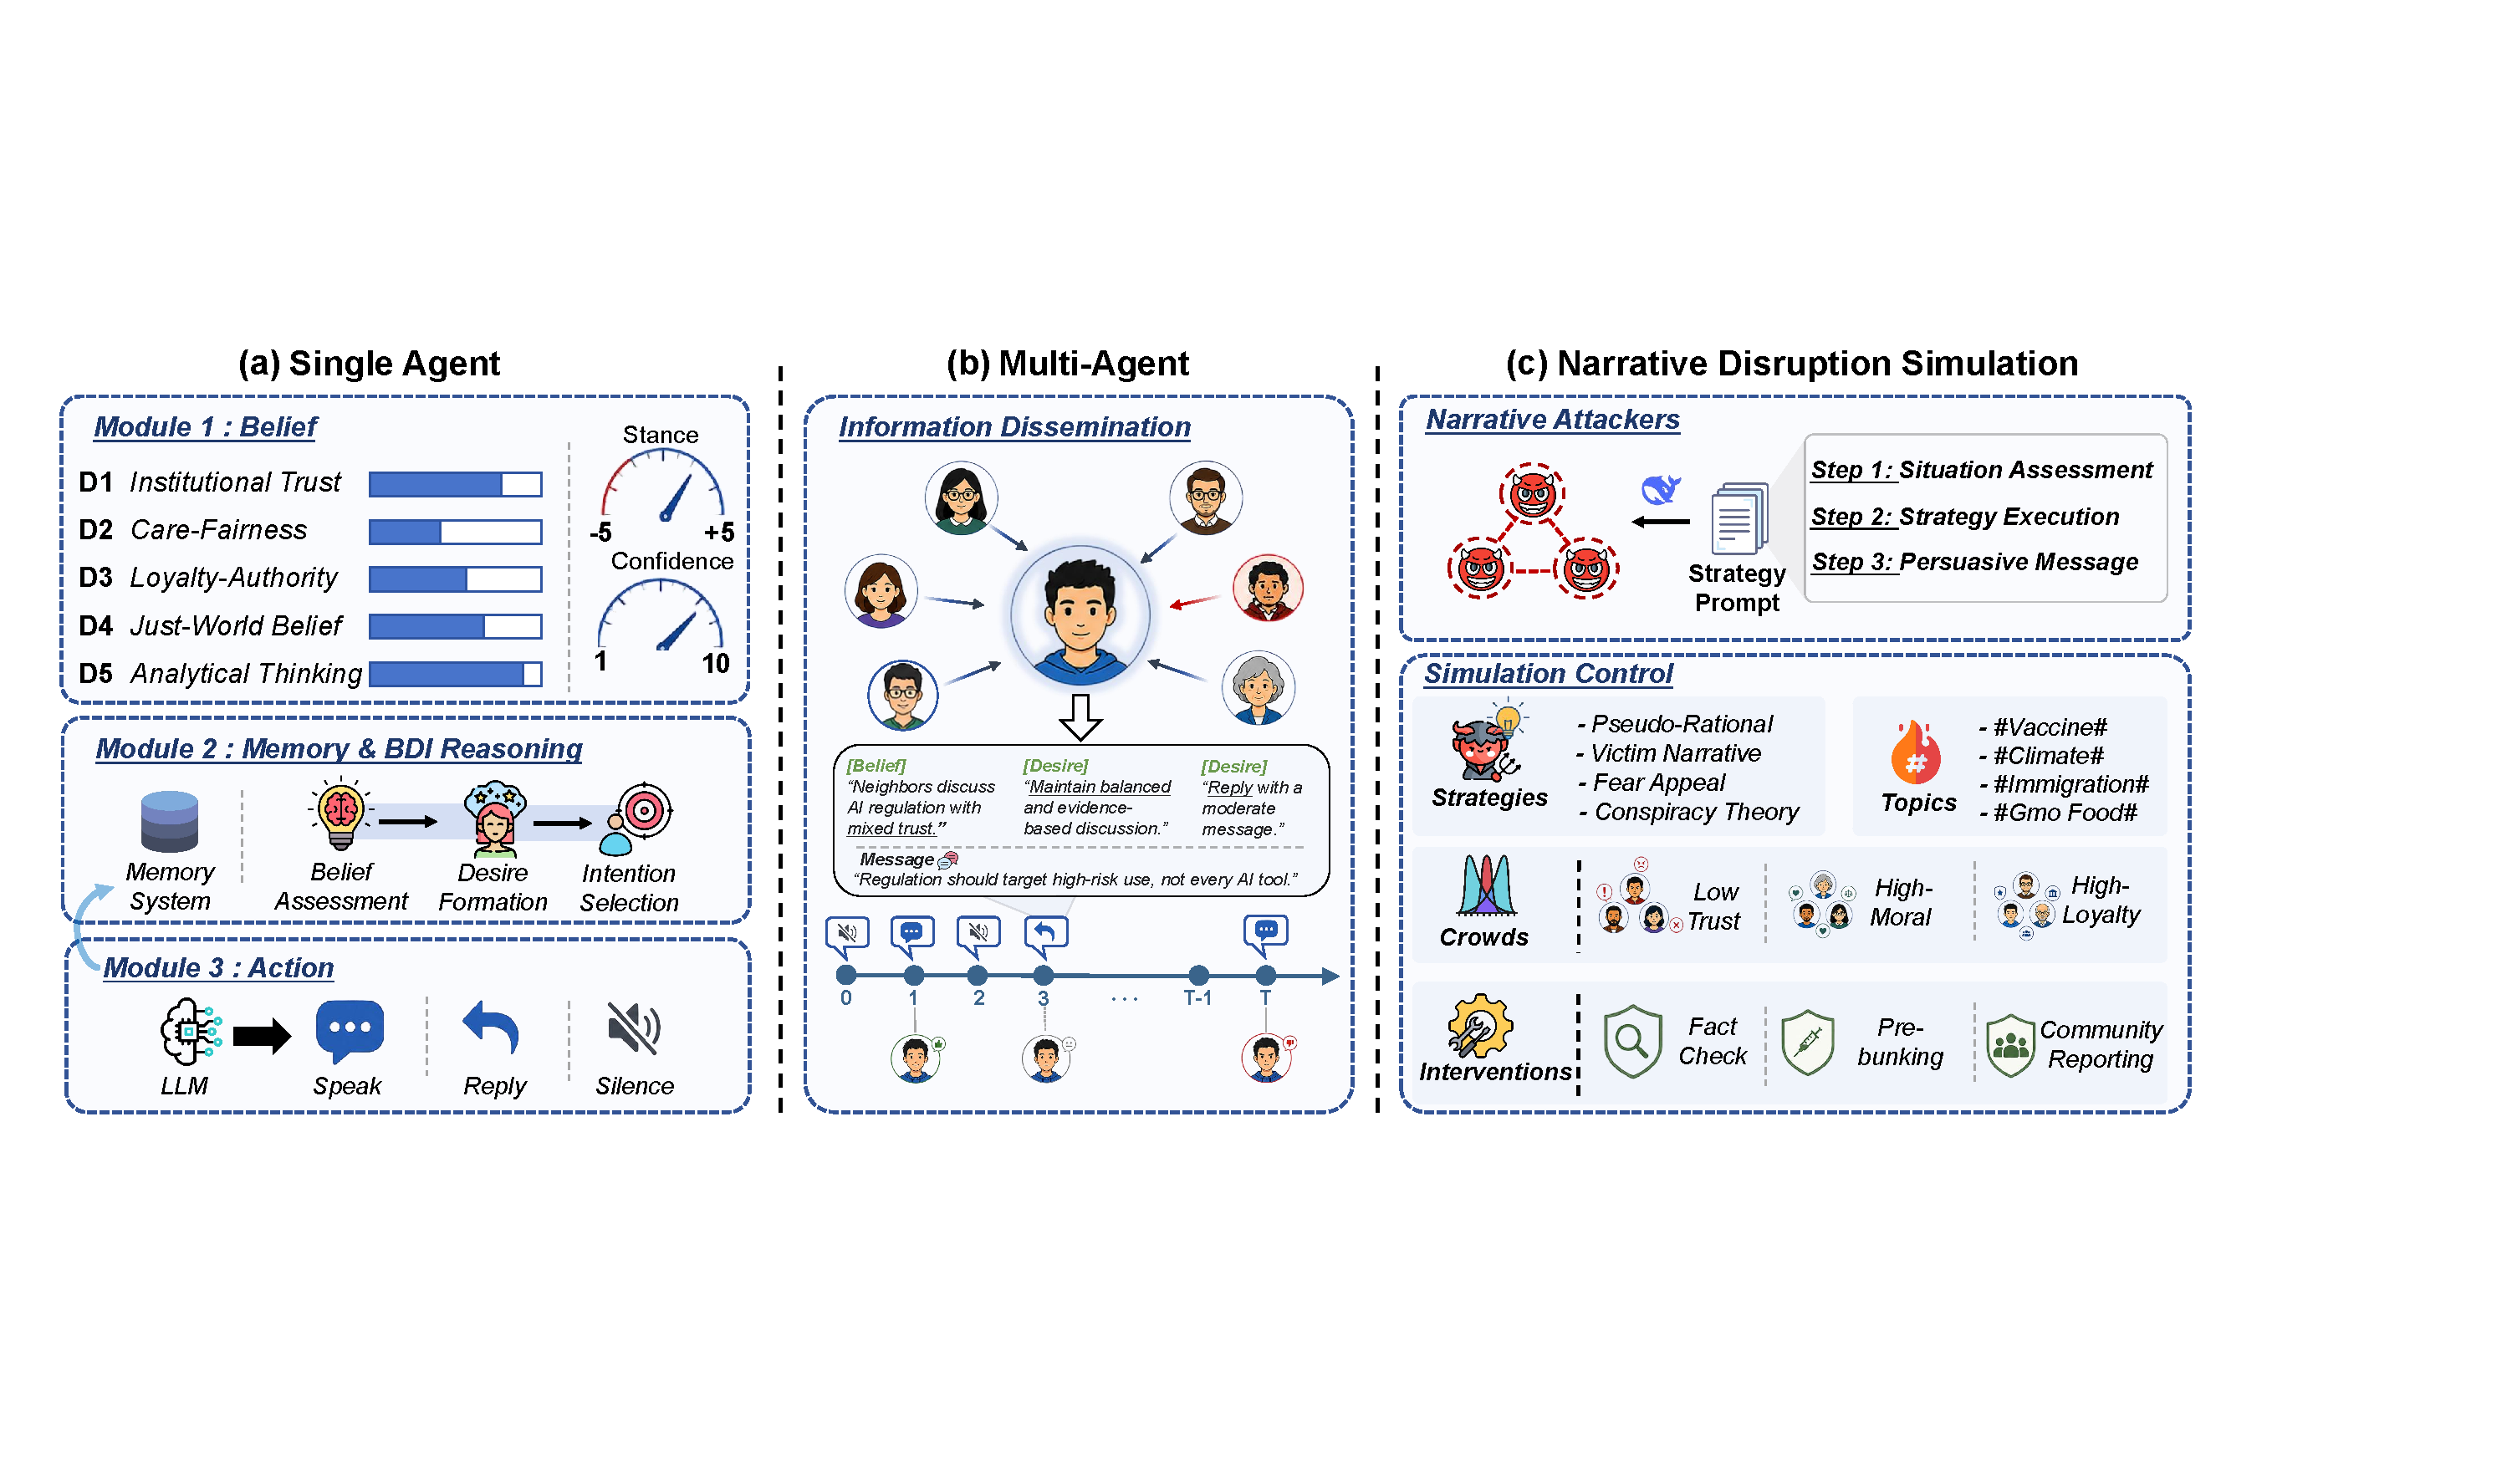
\includegraphics[width=\textwidth]{framework.pdf}
\caption{\textbf{NarrateSim}概览。(a)~普通智能体包含信念模块（五个静态心理维度加上动态立场和信心）、记忆与BDI推理模块，以及输出交际行为的行动模块。(b)~智能体通过同步轮次的局部消息交换在无标度社交网络上进行交互。(c)~完整模拟集成了普通智能体、策略约束的叙事攻击者、可配置干预（预防性接种、事实核查、社区举报），以及跨话题和人口特征的析因实验条件。}
\label{fig:framework}
\end{figure*}

我们用\textbf{NarrateSim}研究此问题——一个将基于LLM的智能体置于争议性话题网络化讨论中的多智能体模拟框架。图~\ref{fig:framework}给出总体概览，本节后续描述智能体架构（\S\ref{sec:agent}）、多智能体交互机制（\S\ref{sec:interaction}）以及叙事攻击者的设计（\S\ref{sec:malicious}）。

\subsection{智能体架构}
\label{sec:agent}

每个普通智能体被建模为具有三个互联模块的认知实体：编码其心理特征和当前意见的\emph{信念模块}、支持结构化BDI推理的\emph{记忆与推理模块}，以及将推理结果映射为交际行为的\emph{行动模块}。

\subsubsection{信念模块}

对错误信息的易感性并非单一特质，而是源于多种认知和倾向性因素的交互~\citep{Ecker2022}。为捕捉这种多维特性，我们为每个智能体配备了结构化信念系统，包含定义持久心理倾向的静态信念维度和在讨论中演化的动态信念状态。

\paragraph{静态信念。}
遵循\citet{Ecker2022}的整合框架，我们操作化了涵盖认知风格、世界观和制度取向的五个维度，每个取值于$[1, 10]$：

\begin{itemize}
\setlength{\itemsep}{1pt}
\item $D_1$，\emph{制度信任}：对政府、媒体和专家的信心~\citep{Mishler2001}。
\item $D_2$，\emph{关怀--公正}：以共情和伤害预防为核心的个体化道德基础~\citep{Graham2013}。
\item $D_3$，\emph{忠诚--权威}：以群体凝聚力和社会秩序为核心的约束性道德基础~\citep{Graham2013, Feinberg2019}。
\item $D_4$，\emph{公正世界信念}：倾向于认为现有体制公平的程度~\citep{Lerner1980}。
\item $D_5$，\emph{分析性思维}：偏向审慎推理而非直觉推理的倾向~\citep{Pennycook2021}。
\end{itemize}

每个维度从可配置的高斯分布中采样。数值向量$\mathbf{D}^{(i)}$随后通过基于规则的映射转换为自然语言人格描述$\mathcal{P}^{(i)}$，以纯文本方式刻画智能体的态度。该描述嵌入智能体的系统提示中，在整个模拟过程中保持不变，使LLM能够基于可解释的性格信息进行推理。

\paragraph{动态信念。}
每个智能体维护两个可变状态：\emph{立场} $s_t^{(i)} \in \{-5, \ldots, +5\}$ 表示其在话题上的位置，以及\emph{信心} $c_t^{(i)} \in \{1, \ldots, 10\}$ 表示对该位置的坚定程度。这种二维表示遵循将位置与确定性分离的意见动力学模型~\citep{FriedkinJohnsen1990}。初始值从可配置分布中采样，并在每轮通过BDI推理过程更新。


\subsubsection{记忆与推理模块}

\paragraph{记忆机制。}
我们配对两种互补的记忆类型用于推理。\emph{情境感知}提供当前社交环境的快照：每轮智能体观察其网络邻居的最新消息。\emph{经验记忆}是一个滑动窗口$\mathcal{M}_t^{(i)}$，存储智能体自身最近$K$轮的记录（$K{=}10$），包括过去的立场、行动和消息，使其能够追踪自身观点的演变并保持自我一致性。

\paragraph{BDI推理。}
在每次发言前，智能体运行受BDI架构~\citep{Bratman1987, Rao1995}启发的结构化推理步骤，我们将其视为信念更新——智能体修正其当前想法、决定要说什么，并承诺如何表达。三个阶段为：
\begin{itemize}
\setlength{\itemsep}{1pt}
\item \textbf{信念}：根据邻居的最新消息和经验记忆中自身的过往立场，更新智能体对话题和周围情绪的看法。
\item \textbf{意愿}：识别智能体感到需要表达的内容，包括在没有新观点时选择沉默。
\item \textbf{意图}：选择具体的交际行动并给出简要理由。
\end{itemize}
推理输出形式化为：
\begin{equation}
\begin{aligned}
  \mathbf{O}_t^{(i)} &= \bigl(a_t^{(i)},\, \tau_t^{(i)},\, s_t^{(i)},\, c_t^{(i)},\, m_t^{(i)}\bigr) \\
  &= f_{\text{LLM}}\bigl(\mathcal{P}^{(i)},\, \mathcal{M}_t^{(i)},\, \mathcal{N}_t^{(i)},\, \mathcal{B}\bigr)
\end{aligned}
\label{eq:bdi_output}
\end{equation}
其中$a_t^{(i)} \in \{\textsc{speak}, \textsc{reply}, \textsc{silent}\}$为行动，$\tau_t^{(i)}$为可选的回复目标，$s_t^{(i)}$和$c_t^{(i)}$为更新后的立场和信心，$m_t^{(i)}$为生成的消息，$\mathcal{B}$表示调节交际规范以近似真实在线话语的行为约束。


\subsubsection{行动模块}

行动模块位于智能体内部推理与社交环境之间，解析结构化的LLM响应以提取所选行动、目标和消息，并针对行为约束进行验证，确保结果与在线平台规范一致。\textsc{speak}或\textsc{reply}将生成的消息广播给邻居并进入其下一轮的情境感知，而\textsc{silent}不贡献消息但仍更新智能体的内部状态。


\subsection{多智能体交互}
\label{sec:interaction}

智能体通过Barab\'{a}si--Albert（BA）优先连接网络~\citep{Barabasi1999}相连，该网络产生无标度拓扑，其中大多数节点连接较少而少数节点作为高连接枢纽，近似真实在线平台的异质连通性。在默认配置（$m{=}3$，$N{=}100$）下，网络产生约6的平均度，且拓扑和随机种子在各条件间保持恒定以隔离操纵变量的效应。模拟进行$T$个同步轮次；每轮每个普通智能体观察其直接邻居的最新消息并通过BDI推理（方程~\ref{eq:bdi_output}）产生响应，这种局部可见性约束使意见通过网络结构逐步传播。


\subsection{叙事攻击者}
\label{sec:malicious}

我们将叙事攻击者建模为自适应对抗性智能体，代表当前常见的协调性在线影响操作~\citep{Ferrara2016}。与广播预写内容的模板式机器人不同，我们的攻击者观察不断演化的讨论，并在每轮生成情境自适应的说服性消息。

\paragraph{策略约束生成。}
每个攻击者由精心设计的策略提示驱动，该提示同时指定其应采用的说服机制和必须避免的策略，防止跨策略污染并确保任何观察到的效果可归因于策略本身。在生成消息前，攻击者对最近的讨论进行简要情况评估，阅读主流情绪，识别哪些参与者对所选角度最易说服，并为该轮选择具体策略。它可以按名字引用特定参与者、回应新出现的论点，并随对话发展调整修辞。

\paragraph{协调与评估。}
每个攻击者被赋予比任何单个普通智能体更广泛的周围智能体视野，包括整个网络的最近消息和主导情绪的粗略摘要。当多个攻击者在同一模拟中行动时，它们在一轮内顺序发帖并阅读队友已发布的内容，这使它们能够采取互补角度并多样化攻击面。叙事攻击者不携带信念维度、不更新立场，并被排除在所有评估指标之外，因此对立场、信心和情绪气候的测量效果仅反映普通群体的变化。实验中使用的具体策略和协调模式见第~\ref{sec:experiments}节。
